\documentclass[sigconf]{acmart}
\usepackage{lmodern}
\usepackage[T1]{fontenc}
\usepackage{graphicx}
\usepackage{amsmath}
\usepackage{algorithm}
\usepackage{algorithmic}
\usepackage{booktabs}
\usepackage{float}
\usepackage{placeins}

\title{Fantasy Football Optimization: An Evolutionary and Swarm Intelligence Approach}
\author{Marco De Rito}
\affiliation{%
	\institution{University of Trieste}
	\city{Trieste}
	\country{Italy}}
\email{marco.derito@studenti.units.it}

\begin{document}
	\maketitle
	
	\begin{abstract}
		This paper presents an evolutionary computation and swarm intelligence approach to optimize fantasy football team selection. The primary objective is to maximize the total team score within predefined budgetary and positional constraints. Particle Swarm Optimization (PSO), Differential Evolution (DE), and Evolution Strategies (ES) algorithms were employed, alongside fuzzy logic for dynamic parameter tuning. Empirical analysis and graphical evaluations from a concrete execution of the developed software demonstrate robust and satisfactory optimization performance.
	\end{abstract}
	
	\keywords{Fantasy Football, Particle Swarm Optimization, Differential Evolution, Evolution Strategies, Fuzzy Logic, Evolutionary Computation, Swarm Intelligence, Data Analysis, Algorithmic Optimization}
	
	\section{Introduction}
	Fantasy football team selection is inherently an optimization problem constrained by player roles, budget limitations, and scoring metrics. Leveraging computational intelligence methodologies, this project explores PSO, DE, and ES to find optimal team compositions.
	
	\section{Background}
	The theoretical foundations include Particle Swarm Optimization (PSO), Differential Evolution (DE), and Evolution Strategies (ES). Each method is extensively employed in optimization problems due to their effectiveness in handling complex, multidimensional search spaces. Additional inspiration comes from fuzzy logic used to dynamically adjust algorithm parameters for improved performance.
	
	\section{Methodology and Approach}
	
	\subsection{Data Preprocessing}
	Player data was carefully preprocessed to compute accurate fantasy scores based on historical football statistics:
	\begin{multline}
		\text{Score} = 0.5\times Goals + 0.2\times Assists - 0.05\times YellowCards \\ - 0.1\times RedCards + 0.2\times FantasyRating + 0.2\times Penalties
	\end{multline}
	Missing data handling and data normalization techniques were applied.
	
	\subsection{Algorithmic Approaches}
	
	\textbf{Particle Swarm Optimization (PSO):} 
	\begin{align}
		v_{id}^{t+1} &= \omega v_{id}^{t} + c_{p} r_{p} (p_{id}^{t} - x_{id}^{t}) + c_{g} r_{g} (g_{d}^{t} - x_{id}^{t}) \\
		x_{id}^{t+1} &= x_{id}^{t} + v_{id}^{t+1}
	\end{align}
	
	\textbf{Differential Evolution (DE):}
	\begin{equation}
		x_{i}^{t+1} = x_{r1}^{t} + F \cdot (x_{r2}^{t} - x_{r3}^{t})
	\end{equation}
	
	\textbf{Evolution Strategies (ES):}
	\begin{equation}
		x_i' = x_i + \sigma_i \cdot N(0,1)
	\end{equation}
	
	A fuzzy logic module was implemented to dynamically tune PSO parameters.
	
	\section{Computational and Software Details}
	The Python software developed for this project includes several modules: data loaders, score calculators, optimization algorithms, auction mechanisms, and reporting functions. Key computational aspects:
	\begin{itemize}
		\item \textbf{Surrogate Models}: Used for computational efficiency.
		\item \textbf{Dynamic Parameter Tuning}: Enabled through fuzzy logic for adaptive optimization.
	\end{itemize}
	
	\section{Empirical Performance Analysis}
	Empirical analysis was conducted through multiple case studies. This paper focuses on a representative concrete execution illustrating performance metrics clearly in Table \ref{tab:performance}:
	
	\begin{table}[H]
		\centering
		\begin{tabular}{lccc}
			\toprule
			Strategy & Managers & Avg Total Score & Avg Team Score \\
			\midrule
			PSO & 4 & 49.40 & 2.95 \\
			DE & 4 & 51.76 & 2.92 \\
			ES & 4 & 44.85 & 2.65 \\
			\bottomrule
		\end{tabular}
		\caption{Strategy Performance Comparison}
		\label{tab:performance}
	\end{table}
	
	\section{Visualization of Data and Results}
	The graphical analyses illustrate the effectiveness of the approach clearly in one concrete execution:
	
	\begin{figure}[H]
		\centering
		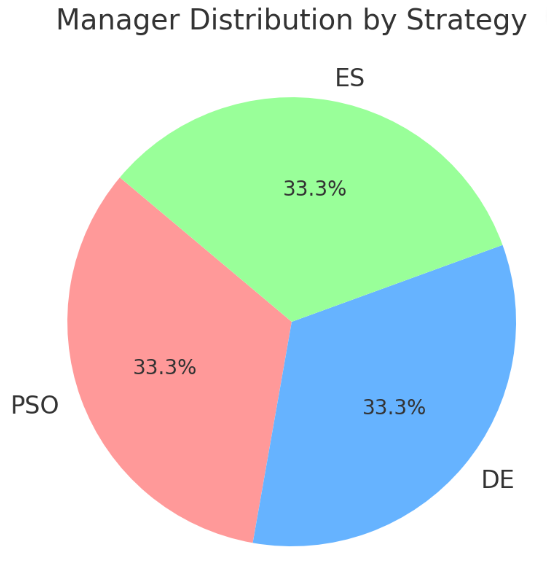
\includegraphics[width=0.9\linewidth]{plot/manager_distribution.png}
		\caption{Manager Distribution by Strategy}
		\label{fig:manager_distribution}
	\end{figure}
	
	\begin{figure}[H]
		\centering
		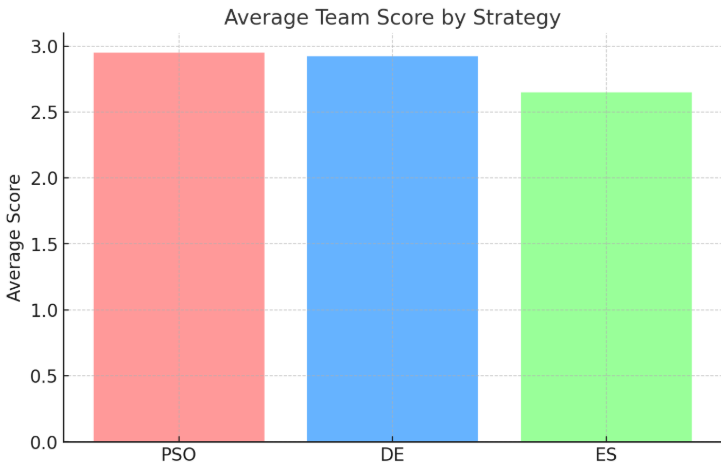
\includegraphics[width=0.9\linewidth]{plot/average_team_score_strategy.png}
		\caption{Average Team Score by Strategy}
		\label{fig:avg_team_score}
	\end{figure}
	
	\begin{figure}[H]
		\centering
		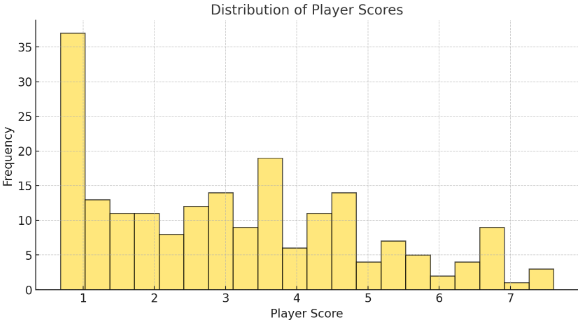
\includegraphics[width=0.9\linewidth]{plot/player_score_distribution.png}
		\caption{Distribution of Player Scores}
		\label{fig:player_score_dist}
	\end{figure}
	
	\begin{figure}[H]
		\centering
		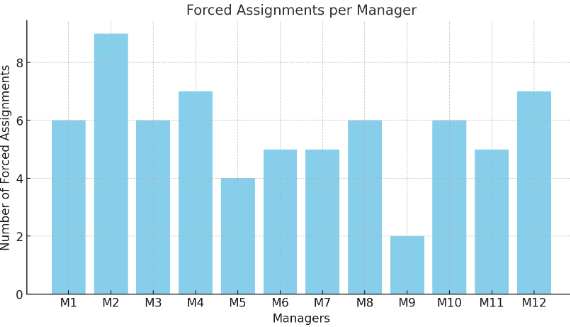
\includegraphics[width=0.9\linewidth]{plot/forced_assignments.png}
		\caption{Forced Assignments per Manager}
		\label{fig:forced_assignments}
	\end{figure}
	
	\begin{figure}[H]
		\centering
		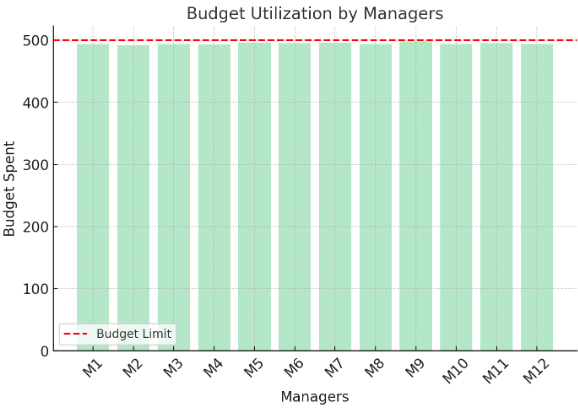
\includegraphics[width=0.9\linewidth]{plot/budget_usage.png}
		\caption{Budget Utilization}
		\label{fig:budget_usage}
	\end{figure}
	
	\section{Discussion \& Conclusion}
	The results from the concrete execution showcase that the DE algorithm achieved the highest overall score, highlighting the importance of robust bidding strategies and adaptive parameter tuning. Overall, the methodologies demonstrated their efficacy and robustness in solving the complex optimization task of fantasy football team selection.
	
	\section{Future Work}
	Future enhancements include:
	\begin{itemize}
		\item Hybridization of optimization techniques
		\item Enhanced real-time data integration
		\item Further exploration into multi-objective optimization approaches
	\end{itemize}
	
	\section*{Acknowledgments}
	Special thanks to the Advanced Optimization Course for the theoretical and practical guidance provided throughout this project.
	
	\bibliographystyle{ACM-Reference-Format}
	\bibliography{references}
	
\end{document}
